\documentclass[a4paper, 12pt]{extreport}
%\usepackage{showframe}
\pdfminorversion=7

\usepackage{rotfloat}
\usepackage{calc}
\usepackage{rotating}

% --- ОСНОВНЫЕ ПАКЕТЫ ---
\usepackage[table]{xcolor}
\usepackage[T2A]{fontenc}
\usepackage[utf8]{inputenc}
\usepackage[english,russian]{babel}
\usepackage{amssymb,amsfonts,amsmath,mathtext,cite,float}
\usepackage{pgfplots}
\pgfplotsset{compat=1.18}
\usepackage{pgf}
\usepackage{graphicx}
\usepackage{tocloft}
\usepackage{listings}
\usepackage{caption}
\usepackage{tempora}
\usepackage{titlesec}
\usepackage{setspace}
\usepackage{geometry}
\usepackage{indentfirst}
\usepackage{pdfpages}
\usepackage{letltxmacro}
\usepackage{threeparttable}
\usepackage{hyperref}
\usepackage{flafter}
\usepackage{enumitem}
\usepackage{multirow}
\usepackage{svg}
\usepackage{makecell}
\usepackage{array}
\usepackage{longtable}
\usepackage{csvsimple}
\usepackage{tikz}
\usetikzlibrary{arrows.meta}

\usepackage{xassoccnt}
\NewTotalDocumentCounter{TotalFigures}
\NewTotalDocumentCounter{TotalTables}
\DeclareAssociatedCounters{figure}{TotalFigures}
\DeclareAssociatedCounters{table}{TotalTables}

% --- СЧЁТЧИКИ ---
\usepackage[figure,table]{totalcount}
\usepackage{lastpage}

% --- СПИСКИ ---
\setlist{nosep}

% --- РАЗДЕЛЫ ---
\newcommand{\ssr}[1]{%
	\begin{center}
		\LARGE\bfseries{#1}
	\end{center}
	\addcontentsline{toc}{chapter}{#1}
}

\makeatletter
\renewcommand\LARGE{\@setfontsize\LARGE{22pt}{20}}
\renewcommand\Large{\@setfontsize\Large{20pt}{20}}
\renewcommand\large{\@setfontsize\large{16pt}{20}}
\makeatother

\RequirePackage{titlesec}
\titleformat{\chapter}[block]{\hspace{\parindent}\large\bfseries}{\thechapter}{0.5em}{\large\bfseries\raggedright}
\titleformat{name=\chapter,numberless}[block]{\hspace{\parindent}}{}{0pt}{\large\bfseries\centering}
\titleformat{\section}[block]{\hspace{\parindent}\large\bfseries}{\thesection}{0.5em}{\large\bfseries\raggedright}
\titleformat{\subsection}[block]{\hspace{\parindent}\large\bfseries}{\thesubsection}{0.5em}{\large\bfseries\raggedright}
\titleformat{\subsubsection}[block]{\hspace{\parindent}\large\bfseries}{\thesubsubsection}{0.5em}{\large\bfseries\raggedright}

\titlespacing{\chapter}{12.5mm}{0pt}{10pt}
\titlespacing{\section}{12.5mm}{10pt}{10pt}
\titlespacing{\subsection}{12.5mm}{10pt}{10pt}
\titlespacing{\subsubsection}{12.5mm}{10pt}{10pt}

% --- БИБЛИОГРАФИЯ ---
\makeatletter
\renewcommand{\@biblabel}[1]{#1.}
\makeatother

% --- ПОЛЯ ---
\geometry{left=30mm, right=10mm, top=20mm, bottom=20mm}
\onehalfspacing

% --- НУМЕРАЦИЯ СПИСКОВ ---
\renewcommand{\theenumi}{\arabic{enumi}}
\renewcommand{\labelenumi}{\arabic{enumi})}
\renewcommand{\theenumii}{\asbuk{enumii}}
\renewcommand{\labelenumii}{\asbuk{enumii})}

\renewcommand{\theenumiii}{\arabic{enumiii}}
\renewcommand{\labelenumiii}{\arabic{enumi}.\arabic{enumii}.\arabic{enumiii}.}

\renewcommand{\cftchapleader}{\cftdotfill{\cftdotsep}}
%\cftsetindents{chapter}{0em}{2.6em}
%\cftsetindents{section}{0em}{2.6em}
%\cftsetindents{subsection}{0em}{2.6em}
%\cftsetindents{subsubsection}{0em}{2.6em}

% --- ПОДПИСИ ---
\addto\captionsrussian{\renewcommand{\figurename}{Рисунок}}
\DeclareCaptionLabelSeparator{dash}{~---~}
\captionsetup{labelsep=dash}
\captionsetup[figure]{justification=centering,labelsep=dash}
\captionsetup[table]{justification=raggedleft,labelsep=dash,singlelinecheck=off}
\captionsetup[lstlisting]{justification=raggedright,singlelinecheck=false}

%\captionsetup[lstlisting]{justification=raggedright, singlelinecheck=false, width=\linewidth}

% --- ПУТЬ К КАРТИНКАМ ---
\graphicspath{{images/}}

% --- МАТЕМАТИКА ---
\newcommand{\floor}[1]{\lfloor #1 \rfloor}

% --- ЛИСТИНГИ ---
\lstset{
	language=caml,
	basicstyle=\small\ttfamily,
	numbers=none,
	numberstyle=\tiny,
	stepnumber=1,
	showspaces=false,
	showstringspaces=false,
	showtabs=false,
	frame=single,
	tabsize=2,
	captionpos=t,
	breaklines=true,
	breakatwhitespace=true,
	columns=fullflexible,
	keepspaces=true,
	escapeinside={\#*}{*)},
	abovecaptionskip=-5pt,
	literate={а}{{\char224}}1 {б}{{\char225}}1 {в}{{\char226}}1 {г}{{\char227}}1 {д}{{\char228}}1 {е}{{\char229}}1
	{ё}{{\char184}}1 {ж}{{\char230}}1 {з}{{\char231}}1 {и}{{\char232}}1 {й}{{\char233}}1 {к}{{\char234}}1 {л}{{\char235}}1
	{м}{{\char236}}1 {н}{{\char237}}1 {о}{{\char238}}1 {п}{{\char239}}1 {р}{{\char240}}1 {с}{{\char241}}1 {т}{{\char242}}1
	{у}{{\char243}}1 {ф}{{\char244}}1 {х}{{\char245}}1 {ц}{{\char246}}1 {ч}{{\char247}}1 {ш}{{\char248}}1 {щ}{{\char249}}1
	{ъ}{{\char250}}1 {ы}{{\char251}}1 {ь}{{\char252}}1 {э}{{\char253}}1 {ю}{{\char254}}1 {я}{{\char255}}1
	{А}{{\char192}}1 {Б}{{\char193}}1 {В}{{\char194}}1 {Г}{{\char195}}1 {Д}{{\char196}}1 {Е}{{\char197}}1
	{Ё}{{\char168}}1 {Ж}{{\char198}}1 {З}{{\char199}}1 {И}{{\char200}}1 {Й}{{\char201}}1 {К}{{\char202}}1 {Л}{{\char203}}1
	{М}{{\char204}}1 {Н}{{\char205}}1 {О}{{\char206}}1 {П}{{\char207}}1 {Р}{{\char208}}1 {С}{{\char209}}1 {Т}{{\char210}}1
	{У}{{\char211}}1 {Ф}{{\char212}}1 {Х}{{\char213}}1 {Ц}{{\char214}}1 {Ч}{{\char215}}1 {Ш}{{\char216}}1 {Щ}{{\char217}}1
	{Ъ}{{\char218}}1 {Ы}{{\char219}}1 {Ь}{{\char220}}1 {Э}{{\char221}}1 {Ю}{{\char222}}1 {Я}{{\char223}}1
	{✓}{{$\checkmark$}}1 {✗}{{$\times$}}1 {—}{{---}}1 {–}{{--}}1
}

\lstdefinestyle{GOSTstyleAppA}{
	basicstyle=\small\ttfamily,
	numbers=left,
	numberstyle=\tiny,
	stepnumber=1,
	numbersep=5pt,
	frame=single,
	breaklines=true,
	tabsize=2,
	captionpos=t,
	keywordstyle=\color{blue},
	commentstyle=\color{gray},
	stringstyle=\color{red},
	showstringspaces=false
}

% --- ПРОЧЕЕ ---
\pgfplotsset{width=0.85\linewidth, height=0.5\columnwidth}
\linespread{1.3}
\parindent=1.25cm

\def\labelitemi{---}
\setlist[itemize]{leftmargin=1.25cm, itemindent=0.65cm}
\setlist[enumerate]{leftmargin=1.25cm, itemindent=0.55cm}

\frenchspacing


\begin{document}
	\thispagestyle{empty}
	
	\noindent \begin{minipage}{0.15\textwidth}
		
\includegraphics[width=\linewidth]{b_logo}
	\end{minipage}
	\noindent\begin{minipage}{0.85\textwidth}\centering
		\textbf{Министерство науки и высшего образования Российской Федерации}\\
		\textbf{Федеральное государственное автономное образовательное учреждение высшего образования}\\
		\textbf{<<Московский государственный технический университет имени Н.Э.~Баумана}\\
		\textbf{(национальный исследовательский университет)>>}\\
		\textbf{(МГТУ им. Н.Э.~Баумана)}
	\end{minipage}
	
	\noindent\rule{\linewidth}{3pt}
	\newline\newline
	\noindent ФАКУЛЬТЕТ $\underline{\text{<<Информатика и системы управления>>}}$ \newline\newline
	\noindent КАФЕДРА $\underline{\text{<<Программное обеспечение ЭВМ и информационные технологии>>}}$
	
	\vspace{1cm}
	
	\begin{center}
		\noindent\begin{minipage}{1.3\textwidth}\centering
			\Large\textbf{  Лабораторная работа}\newline
			\textbf{по дисциплине <<Операционные системы>>}\newline\newline
		\end{minipage}
	\end{center}
	
	\noindent\textbf{Тема} $\underline{\text{Буферизованный и небуферизованный ввод-вывод}}$\newline\newline
	\noindent\textbf{Студент} $\underline{\text{Палладий~Е.~И.}}$\newline\newline
	\noindent\textbf{Группа} $\underline{\text{ИУ7-61Б}}$\newline\newline
	\noindent\textbf{Преподаватели} $\underline{\text{Рязанова~Н.~Ю.}}$\newline
	
	\begin{center}
		\vfill
		Москва,~\the\year
	\end{center}
	\clearpage
	\chapter{Структуры}
	
	\section{FILE и структура \_IO\_FILE}
	
	\begin{lstlisting}[caption={FILE /libio/bits/types/FILE.h}, label={code:file}]
		#ifndef __FILE_defined
		#define __FILE_defined 1
		struct _IO_FILE;
		/* The opaque type of streams.  This is the definition used elsewhere.  */
		typedef struct _IO_FILE FILE;
		#endif
	\end{lstlisting}
	
	\begin{lstlisting}[caption={\_IO\_FILE /libio/bits/types/struct\_FILE.h}, label={code:iofile}]
		struct _IO_FILE
		{
			int _flags;		/* High-order word is _IO_MAGIC; rest is flags. */
			
			/* The following pointers correspond to the C++ streambuf protocol. */
			char *_IO_read_ptr;	/* Current read pointer */
			char *_IO_read_end;	/* End of get area. */
			char *_IO_read_base;	/* Start of putback+get area. */
			char *_IO_write_base;	/* Start of put area. */
			char *_IO_write_ptr;	/* Current put pointer. */
			char *_IO_write_end;	/* End of put area. */
			char *_IO_buf_base;	/* Start of reserve area. */
			char *_IO_buf_end;	/* End of reserve area. */
			
			/* The following fields are used to support backing up and undo. */
			char *_IO_save_base; /* Pointer to start of non-current get area. */
			char *_IO_backup_base;  /* Pointer to first valid character of backup area */
			char *_IO_save_end; /* Pointer to end of non-current get area. */
			
			struct _IO_marker *_markers;
			
			struct _IO_FILE *_chain;
			
			int _fileno;
			int _flags2:24;
			/* Fallback buffer to use when malloc fails to allocate one.  */
			char _short_backupbuf[1];
			__off_t _old_offset; /* This used to be _offset but it's too small.  */
			
			/* 1+column number of pbase(); 0 is unknown. */
			unsigned short _cur_column;
			signed char _vtable_offset;
			char _shortbuf[1];
			
			_IO_lock_t *_lock;
			#ifdef _IO_USE_OLD_IO_FILE
		};
		
		struct _IO_FILE_complete
		{
			struct _IO_FILE _file;
			#endif
			__off64_t _offset;
			/* Wide character stream stuff.  */
			struct _IO_codecvt *_codecvt;
			struct _IO_wide_data *_wide_data;
			struct _IO_FILE *_freeres_list;
			void *_freeres_buf;
			struct _IO_FILE **_prevchain;
			int _mode;
			#if __WORDSIZE == 64
			int _unused3;
			#endif
			__uint64_t _total_written;
			#if __WORDSIZE == 32
			int _unused3;
			#endif
			/* Make sure we don't get into trouble again.  */
			char _unused2[12 * sizeof (int) - 5 * sizeof (void *)];
		};
	\end{lstlisting}
	
	\section{Структура stat}
	
	%\vspace*{-2cm}
	\begin{lstlisting}[caption={struct stat}, label={code:stat}]
		struct stat {
			dev_t     st_dev;     /* устройство */
			ino_t     st_ino;     /* inode */
			mode_t    st_mode;    /* режим доступа */
			nlink_t   st_nlink;   /* количество жестких ссылок */
			uid_t     st_uid;     /* идентификатор пользователя-владельца */
			gid_t     st_gid;     /* идентификатор группы-владельца */
			dev_t     st_rdev;    /* тип устройства (если это устройство)*/
			off_t     st_size;    /* общий размер в байтах */
			blksize_t st_blksize; /* размер блока ввода-вывода в файловой системе */
			blkcnt_t  st_blocks;  /* количество выделенных 512-байтных блоков */
			union { time_t st_atime; struct timespec st_atim; }; /* время последнего доступа */
			union { time_t st_mtime; struct timespec st_mtim; }; /* время последней модификации */
			union { time_t st_ctime; struct timespec st_ctim; }; /* время последнего изменения */
		};
	\end{lstlisting}
	
	\newpage
	\chapter{Программа №1}
	
	\section{Код программы}
	
	\begin{lstlisting}[caption={Код первой программы}, label={code:p1}]
	#include <stdio.h>
	#include <fcntl.h>
	
	int main()
	{
		int fd = open("alphabet.txt", O_RDONLY);
		
		FILE *fs1 = fdopen(fd, "r");
		char buff1[20];
		setvbuf(fs1, buff1, _IOFBF, 20);
		
		FILE *fs2 = fdopen(fd, "r");
		char buff2[20];
		setvbuf(fs2, buff2, _IOFBF, 20);
		
		int flag1 = 1, flag2 = 2;
		while(flag1 == 1 || flag2 == 1)
		{
			char c;
			flag1 = fscanf(fs1, "%c", &c);
			if (flag1 == 1) 
			{
				fprintf(stdout, "%c", c);
			}
			flag2 = fscanf(fs2, "%c", &c);
			if (flag2 == 1)
			{ 
				fprintf(stdout, "%c", c); 
			}
		}
		return 0;
	}
	\end{lstlisting}
	
	\section{Результат работы программы}
	
	\begin{figure}[H]
		\centering
		
\includegraphics[width=1\textwidth]{p1}
		\caption{Результат работы первой программы}
		\label{pic:p1}
	\end{figure}
	
	\section{Анализ работы программы}
	
	Системный вызов open открывает файл alphabet.txt в режиме <<только для чтения>>, создаёт структуру file. Ссылка на эту структуру помещается в таблицу файловых дескрипторов процесса. Поскольку дескрипторы 0, 1 и 2 заняты стандартными потоками ввода-вывода, системный вызов возвращает наименьший свободный дескриптор (3), который присваивается переменной fd.
	
	Библиотечной функции fdopen передается дескриптор fd и режим доступа <<только для чтения>>. Функция возвращает указатель на инициализированную структуру FILE, где полю \_fileno присваивается значение fd.
	
	Функция setvbuf задаёт размер буфера 20 байт для fs1 и fs2.
	
	Функция fscanf для fs1 обнаруживает, что буфер пуст, и выполняет системный вызов read, который считывает 20 символов (<<a>>---<<t>>) из файла <<alphabet.txt>> в буфер buff1. При этом значение поля f\_pos структуры file в ядре увеличивается на 20. Затем из буфера извлекается первый символ (<<a>>), записывается в переменную c, а указатель \_IO\_read\_ptr в структуре \_IO\_FILE сдвигается на 1 байт. Вызов fprintf выводит этот символ в стандартный поток вывода.
	
	
	Так как структуры \_IO\_FILE fs1 и fs2 содержат одинаковое значение поля \_fileno и, следовательно, ссылаются на одну и ту же структуру file в ядре, где f\_pos уже равно 20, то при вызове fscanf для fs2 системный вызов read считывает оставшиеся 6 символов (<<u>>---<<z>>) в буфер buff2. Первый символ из буфера fs2 (<<u>>) записывается в переменную c и выводится в стандартный поток вывода.
	
	В последующих итерациях цикла поочерёдно будут выводиться символы из буферов fs1 и fs2.
	Когда будет достигнут конец буфера fs2 (сравняются указатели \_IO\_read\_ptr и \_IO\_read\_end), то программа продолжит выводить оставшиеся символы только из буфера fs1 (вплоть до t), пока не будет достигнут конец буфера fs1.
	
	\section{Иллюстрация связи структур}
	
	\begin{figure}[H]
		\centering
		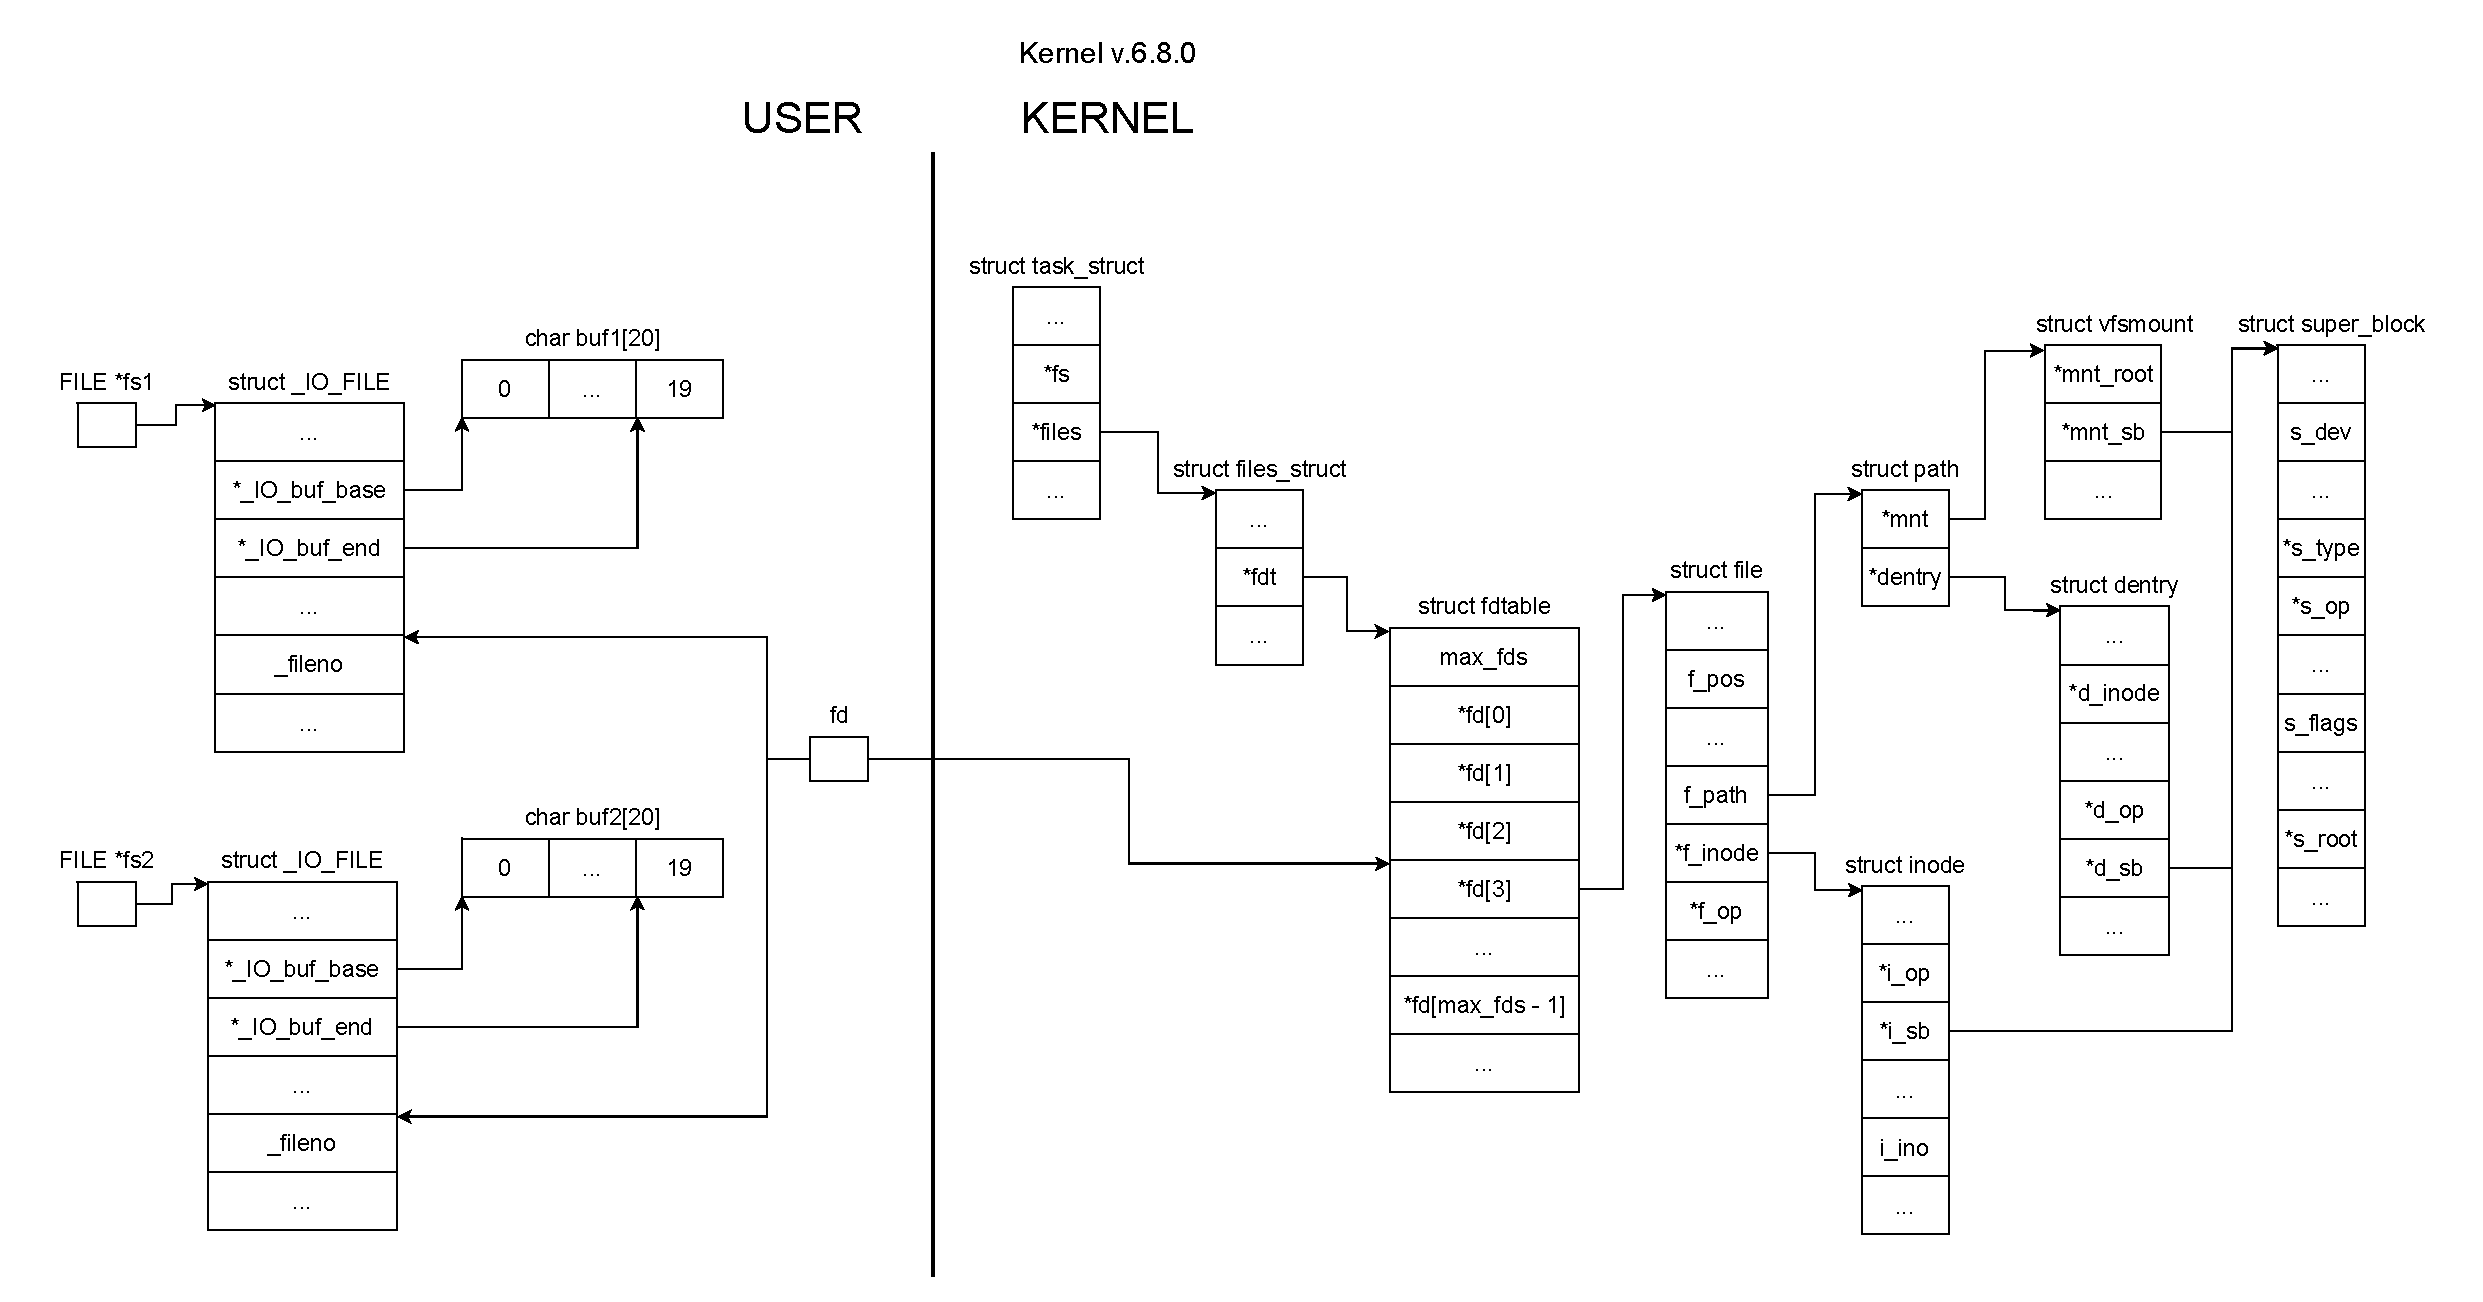
\includegraphics[width=1\textwidth]{1.pdf}
		\caption{Иллюстрация связи структур в первой программе}
		\label{pic:scheme_1}
	\end{figure}
	
	\newpage
	\chapter{Программа №2}
	
	\section{Однопоточный вариант программы}
	
	\subsection{Код программы}
	
	\begin{lstlisting}[caption={Код однопоточной первой программы}, label={code:p2_1thread}]
	#include <fcntl.h>
	#include <unistd.h>
	
	int main()
	{
		char c;
		int fl1 = 1, fl2 = 1; 
		
		int fd1 = open("alphabet.txt", O_RDONLY);
		int fd2 = open("alphabet.txt", O_RDONLY);
		
		while((fl1 == 1) && (fl2 == 1))
		{
			if ((fl1 = read(fd1, &c, 1)) == 1)
			{
				write(1, &c, 1);
			}
			
			if (fl1 == 1 && ((fl2 = read(fd2, &c, 1)) == 1))
			{
				write(1, &c, 1);
			}
		}
		return 0;
	}
	\end{lstlisting}
	
	\subsection{Результат работы программы}
	
	\begin{figure}[H]
		\centering
		
\includegraphics[width=1\textwidth]{p2_read_1thread}
		\caption{Результат работы однопоточной второй программы}
		\label{pic:p1}
	\end{figure}
	
	\subsection{Анализ работы программы}
	
	Системный вызов open создаёт два дескриптора открытого файла в режиме <<только для чтения>> (fd1, fd2). Соответствующие дескрипторам структуры file ссылаются на один и тот же inode файла <<alphabet.txt>>. Ссылки на эти структуры помещаются в таблицу открытых процессом файлов под индексами 3 и 4, так как дескрипторы 0,1 и 2 заняты стандартными потоками.
	
	Системный вызов read для дескриптора fd1 считывает один символ (<<a>>), что приводит к увеличению на 1 значения поля f\_pos в соответствующей структуре file. Считанный символ выводится в стандартный поток вывода.
	
	Так как дескрипторам fd1 и fd2 соответствуют независимые структуры file, то для fd2 значение поля f\_pos равно 0. Поэтому при вызове read для fd2 будет считан тот же самый первый символ (<<a>>), который также выведется в стандартный поток вывода.
	
	Поочерёдное чтение и вывод символов будут продолжаться в цикле, пока значения f\_pos в обеих структурах file не достигнут конца файла (размера файла, хранящегося в поле i\_size и равного 26 байтам).
	
	Таким образом, в стандартный поток вывода каждый символ алфавита будет выведен строго последовательно дважды.
	
	\section{Вариант программы с 1 дополнительным потоком}
	
	\subsection{Код программы}
	
	\begin{lstlisting}[caption={Код программы с 1 дополнительным потоком}, label={code:p2_2thread_join}]
	#include <fcntl.h>
	#include <pthread.h>
	#include <unistd.h>
	#include <stdio.h>
	#include <stdlib.h>
	
	void *thread_func(void *arg)
	{
		char c;
		int fl = 1;
		int fd = *((int *)arg);
		
		while (fl == 1)
		{
			if ((fl = read(fd, &c, 1)))
			write(1, &c, 1);
		}
		return NULL;
	}
	
	int main()
	{
		pthread_t t;
		char c;
		int fl = 1;
		
		int fd1 = open("alphabet.txt", O_RDONLY);
		int fd2 = open("alphabet.txt", O_RDONLY);
		
		if (pthread_create(&t, NULL, thread_func, &fd1) != 0)
		{
			perror("pthread_create");
			exit(1);
		}
		
		while (fl == 1)
		{
			if ((fl = read(fd2, &c, 1)) == 1)
			write(1, &c, 1);
		}
		pthread_join(t, NULL);
		return 0;
	}
	\end{lstlisting}
	
	\subsection{Результат работы программы}
	
	\begin{figure}[H]
		\centering
		
\includegraphics[width=1\textwidth]{p2_read_2thread_join}
		\caption{Результат работы программы с 1 дополнительным потоком}
		\label{pic:p1}
	\end{figure}
	
	\subsection{Анализ работы программы}
	
	Вызов pthread\_create создаёт дополнительный поток, которому в качестве аргумента передаётся указатель на дескриптор fd1. Поскольку на создание потока требуется время, главный поток может успеть прочитать и вывести либо весь алфавит, либо его часть.
	
	После создания дополнительного потока чтение и вывод символов осуществляются обоими потоками в зависящей от планировщика последовательности.
	
	Когда главный поток завершит чтение по своему дескриптору, он выйдет из цикла и заблокируется в вызове pthread\_join, ожидая завершения дополнительного потока. Дополнительный поток продолжит работу и выведет оставшуюся часть своих символов.
	
	Таким образом, каждый символ файла будет напечатан дважды, однако точный порядок их вывода не определён и полностью зависит от того, как планировщик распределяет процессорное время между потоками.
	
	\section{Вариант программы с 2 дополнительными потоками}
	
	\subsection{Код программы}
	
	\begin{lstlisting}[caption={Код программы с 2 дополнительными потоками}, label={code:p2_3thread_join}]
		#include <fcntl.h>
		#include <pthread.h>
		#include <unistd.h>
		#include <stdio.h>
		#include <stdlib.h>
		
		void *thread_func(void *arg)
		{
			char c;
			int fl = 1;
			int fd = *((int *)arg);
			
			while (fl == 1)
			{
				if ((fl = read(fd, &c, 1)))
				write(1, &c, 1);
			}
			return NULL;
		}
		
		int main()
		{
			pthread_t t1, t2;
			
			int fd1 = open("alphabet.txt", O_RDONLY);
			int fd2 = open("alphabet.txt", O_RDONLY);
			
			if (pthread_create(&t1, NULL, thread_func, &fd1) != 0)
			{
				perror("pthread_create");
				exit(1);
			}
			if (pthread_create(&t2, NULL, thread_func, &fd2) != 0)
			{
				perror("pthread_create");
				exit(1);
			}
			
			pthread_join(t1, NULL);
			pthread_join(t2, NULL);
			
			return 0;
		}
	\end{lstlisting}
	
	\subsection{Результат работы программы}
	
	\begin{figure}[H]
		\centering
		
\includegraphics[width=1\textwidth]{p2_read_3thread_join}
		\caption{Результат работы программы с 2 дополнительными потоками}
		\label{pic:p1}
	\end{figure}
	
	\subsection{Анализ работы программы}
	
	Два вызова pthread\_create создают два дополнительных потока. Каждому из них передаётся указатель на свой файловый дескриптор (первому --- fd1, второму --- fd2). Главный поток, создав рабочие потоки, сразу же блокируется в вызовах pthread\_join, ожидая их завершения.
	
	На создание потоков требуется время и их порядок выполнения зависит от планировщика, поэтому порядок вывода символов неизвестен.
	
	Таким образом, каждый символ файла будет напечатан дважды, однако точный порядок их вывода не определён и полностью зависит от того, как планировщик распределяет процессорное время между дополнительными потоками.
	
	\section{Иллюстрация связи структур}
	
	\begin{figure}[H]
		\centering
		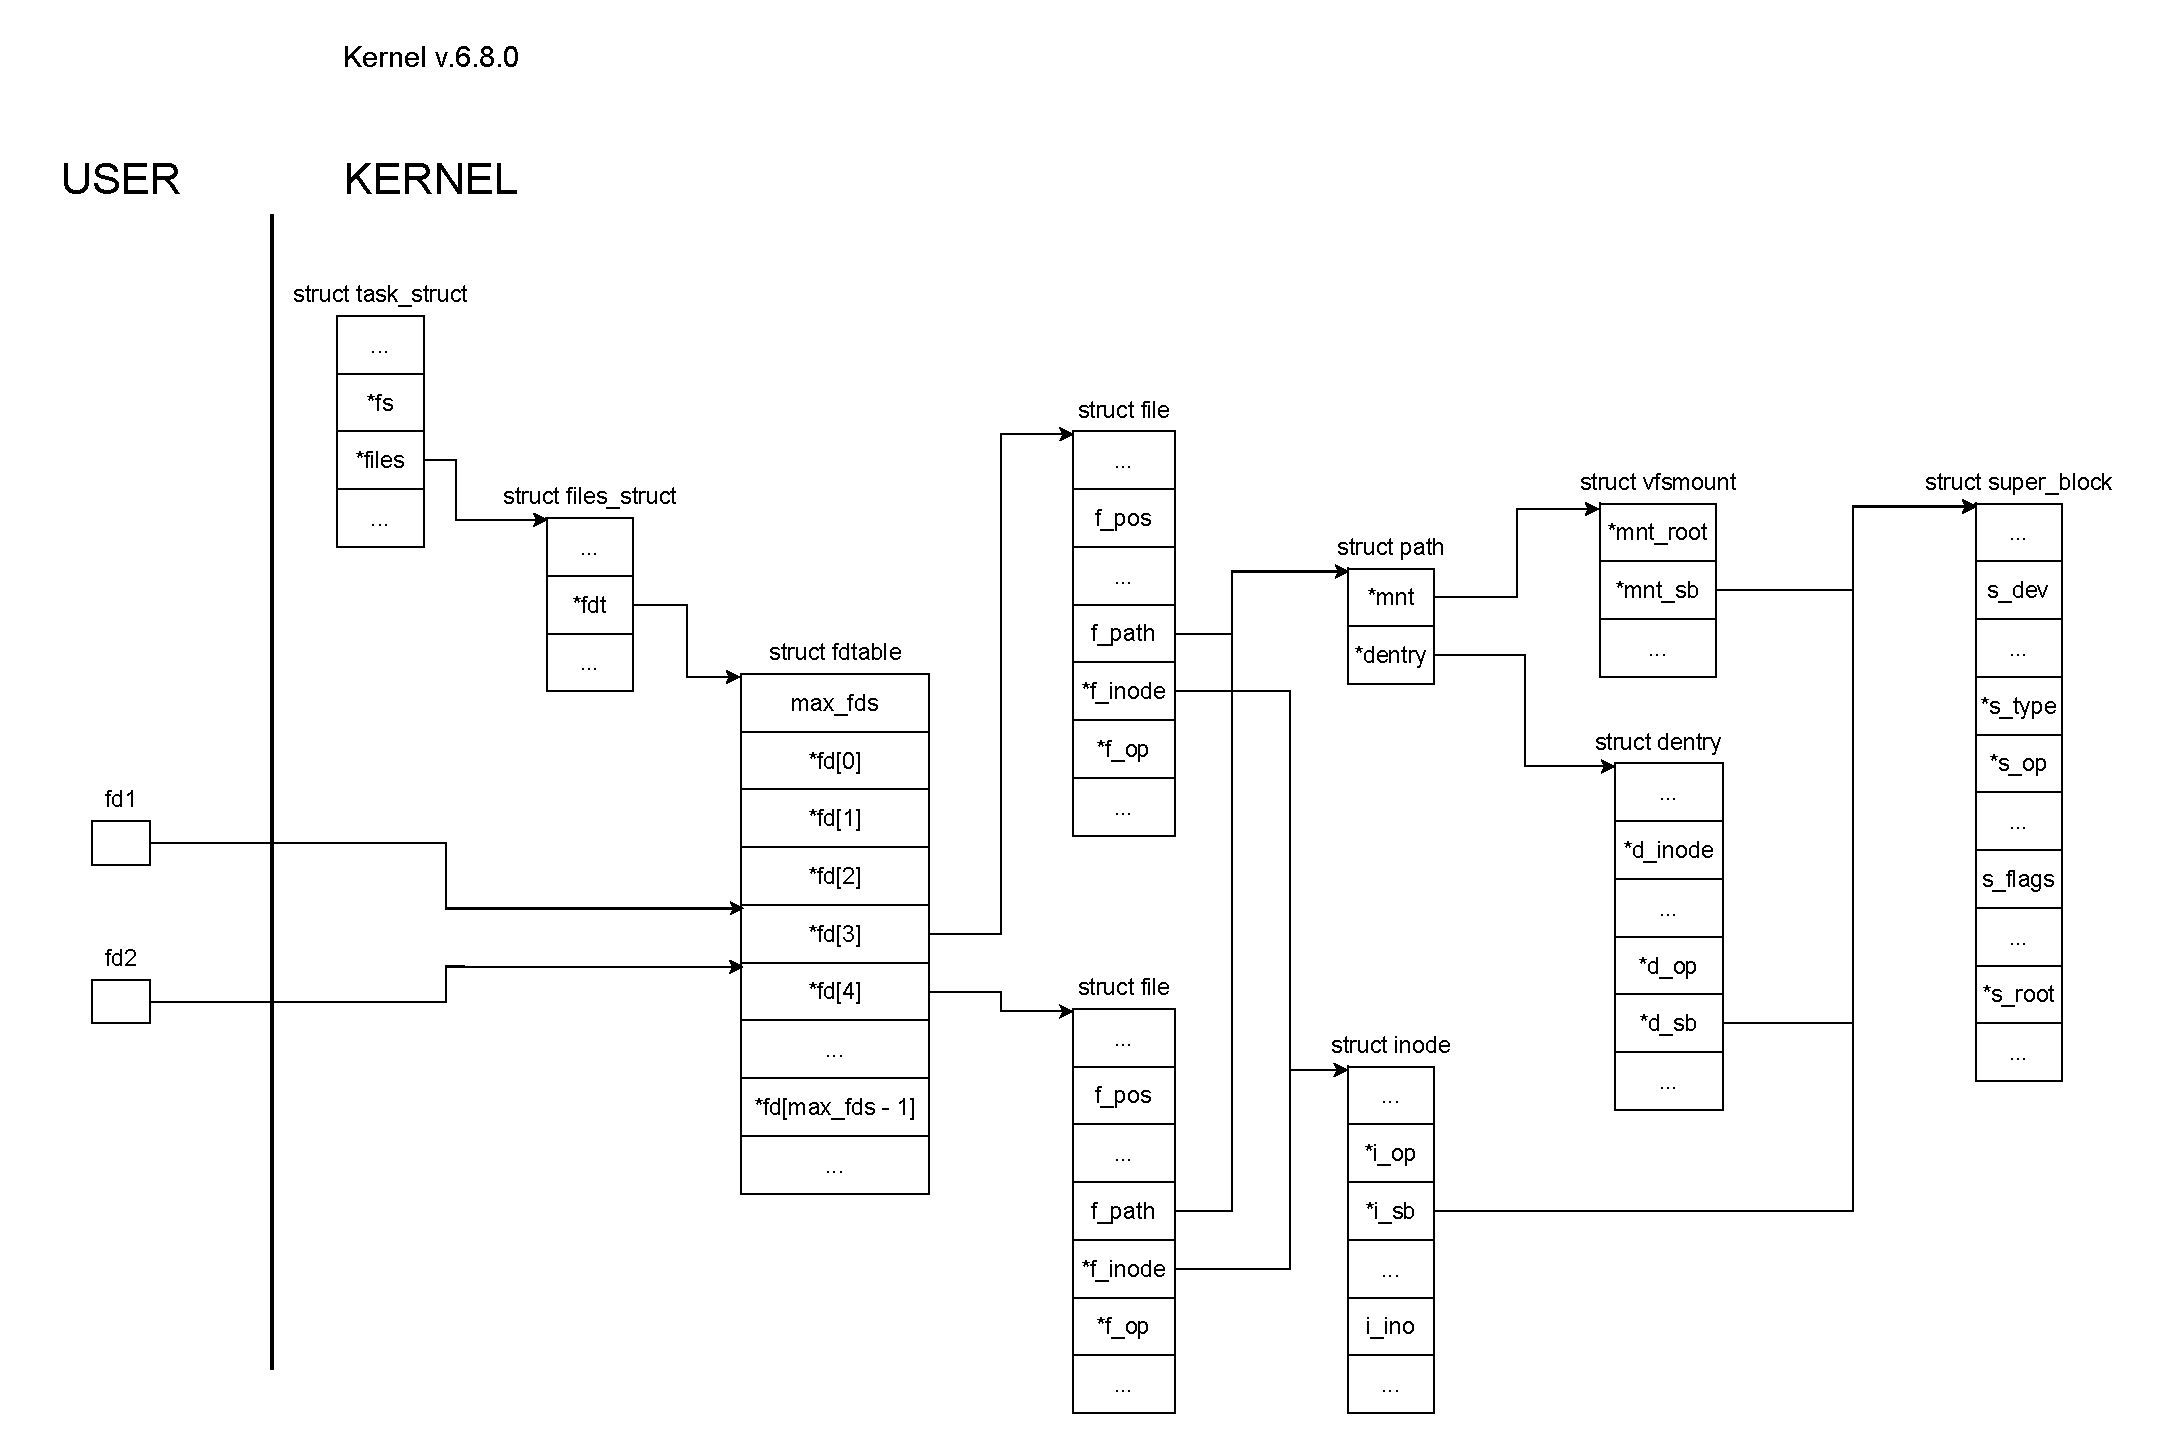
\includegraphics[width=1\textwidth]{2.pdf}
		\caption{Иллюстрация связи структур во второй программе}
		\label{scheme_2}
	\end{figure}
	
	\newpage
	\chapter{Программа №3}
	
	\section{Вариант программы с open, write и close}
	
	\subsection{Код программы}
	
	\begin{lstlisting}[caption={Код программы с open, write и close}, label={code:p3_write}]
	#include <fcntl.h>
	#include <stdio.h>
	#include <unistd.h>
	#include <sys/stat.h>
	#include <sys/types.h>
	
	int main() 
	{
		struct stat statbuf;
		int fd1 = open("q.txt", O_RDWR);
		int fd2 = open("q.txt", O_RDWR);
		stat("q.txt", &statbuf);
		printf("inode: %lu;size: %ld; blksize: %ld\n", statbuf.st_ino, statbuf.st_size, statbuf.st_blksize);
		
		for(char c = 'a'; c <= 'z'; c++)
		{
			if (c%2)
			write(fd1, &c, 1);
			else
			write(fd2, &c, 1);
			stat("q.txt", &statbuf);
			printf("inode: %lu;size: %ld; blksize: %ld\n", statbuf.st_ino, statbuf.st_size, statbuf.st_blksize);
		}
		close(fd1);
		close(fd2);
		return 0;
	}
	\end{lstlisting}
	
	\subsection{Результат работы программы}
	
	\begin{figure}[H]
		\centering
		
\includegraphics[width=1\textwidth]{p3_write}
		\caption{Результат работы программы с open, write и close}
		\label{pic:p3_write}
	\end{figure}
	
	\section{Анализ работы программы}
	
	Системный вызов open создаёт два дескриптора открытого файла в режиме <<чтения и записи>> (fd1, fd2). Соответствующие дескрипторам структуры file ссылаются на один и тот же inode файла <<q.txt>>. Ссылки на эти структуры помещаются в таблицу открытых процессом файлов под индексами 3 и 4, так как дескрипторы 0, 1 и 2 заняты стандартными потоками.
	
	В первой итерации цикла системный вызов write для дескриптора fd1 записывает символ <<a>> в открытый файл, что приводит к увеличению на 1 значения поля f\_pos в соответствующей структуре file. Размер файла становится равным 1 байту.
	
	Так как дескрипторам fd1 и fd2 соответствуют независимые структуры file, то для fd2 значение поля f\_pos остаётся равным 0. Поэтому на второй итерации цикла вызов write для fd2 заменит символ <<a>> в файле на символ <<b>>. Размер файла остаётся равным 1 байту, а значение f\_pos для fd2 увеличится на 1.
	
	Поочерёдная запись символов в файл продолжается до конца цикла.
	
	Таким образом, в файл будет записана только каждая вторая буква алфавита, начиная с <<b>>, и итоговый размер файла составит 13 байт, так как вызов write для fd2 будет заменять символы, записанные вызовом write для fd1.
	
	\section{Иллюстрация связи структур}
	
	Иллюстрация связи структур представлена на рисунке~\ref{pic:scheme_2}.
	
	\section{Вариант программы с fopen, fprintf и fclose}
	
	\subsection{Код программы}
	
	\begin{lstlisting}[caption={Код программы с fopen, fprintf и fclose}, label={code:p3_write}]
	#include <fcntl.h>
	#include <stdio.h>
	#include <sys/stat.h>
	#include <sys/types.h>
	
	int main() 
	{
		struct stat statbuf;
		FILE *fs1 = fopen("q.txt", "w");
		FILE *fs2 = fopen("q.txt", "w");
		stat("q.txt", &statbuf);
		printf("inode: %lu;size: %ld; blksize: %ld\n", statbuf.st_ino, statbuf.st_size, statbuf.st_blksize);
		
		for(char c = 'a'; c <= 'z'; c++)
		{
			if (c%2)
			fprintf(fs1, "%c", c);
			else
			fprintf(fs2, "%c", c);
		}
		stat("q.txt", &statbuf);
		printf("inode: %lu;size: %ld; blksize: %ld\n", statbuf.st_ino, statbuf.st_size, statbuf.st_blksize);
		fclose(fs2);
		fclose(fs1);
		stat("q.txt", &statbuf);
		printf("inode: %lu;size: %ld; blksize: %ld\n", statbuf.st_ino, statbuf.st_size, statbuf.st_blksize);
		return 0;
	}
	\end{lstlisting}
	
	\subsection{Результат работы программы}
	
	\begin{figure}[H]
		\centering
		
\includegraphics[width=1\textwidth]{p3_fprintf}
		\caption{Результат работы программы с fopen, fprintf и fclose}
		\label{pic:p3_fprintf}
	\end{figure}
	
	\subsection{Анализ работы программы}
	
	Вызов библиотечной функции fopen откроет файл <<q.txt>> в режиме <<только для записи с усечением>> и вернёт два указателя на инициализированные структуры FILE (fs1, fs2). Во время вызова создаются две незваисимые структуры file с дескрипторами 3 и 4, значения которых будут записаны в поля \_fileno соотвествующих структур \_IO\_FILE. Эти структуры file ссылаются на один и тот же inode файла <<q.txt>>.
	
	Вызов библиотечной функции fprintf для fs1 записывает символ <<a>> в буфер, что приводит к смещению в соответствующей структуре указателя \_IO\_WRITE\_PTR на 1 байт.
	
	Вызов библиотечной функции fprintf для fs2 записывает символ <<b>> в буфер, что приводит к смещению в соответствующей структуре указателя \_IO\_WRITE\_PTR на 1 байт.
	
	В результате работы цикла в буфере fs1 будет находиться каждая вторая буква алфавита, начиная с <<a>>, а в fs2 --- каждая вторая буква алфавита, начиная с <<b>>.
	
	Вызов fclose для fs2 приводит к записи из буфера в открытый файл. Значение поля f\_pos для дескриптора 4 и размера файла становится 13. После этого дескриптор закрывается.
	
	Так как были созданы две структуры открытых файлов, ссылающихся на один и тот же inode, а в структуре, соответствующей fs1, значение поля f\_pos осталось равным 0, то при вызове fclose для fs1 буфер записывается в открытый файл с начала, что приводит к замене последовательности символов буфера fs2 на последовательность символов буфера fs1. Размер файла остаётся неизменным (13 байт).
	
	Таким образом, итоговое содержимое файла зависит от порядка вызовов fclose. В данном случае в файл будет записан каждый второй символ алфавита, начиная с буквы <<a>>, а размер файла составит 13 байт.
	
	\subsection{Иллюстрация связи структур}
	
	\begin{figure}[H]
		\centering
		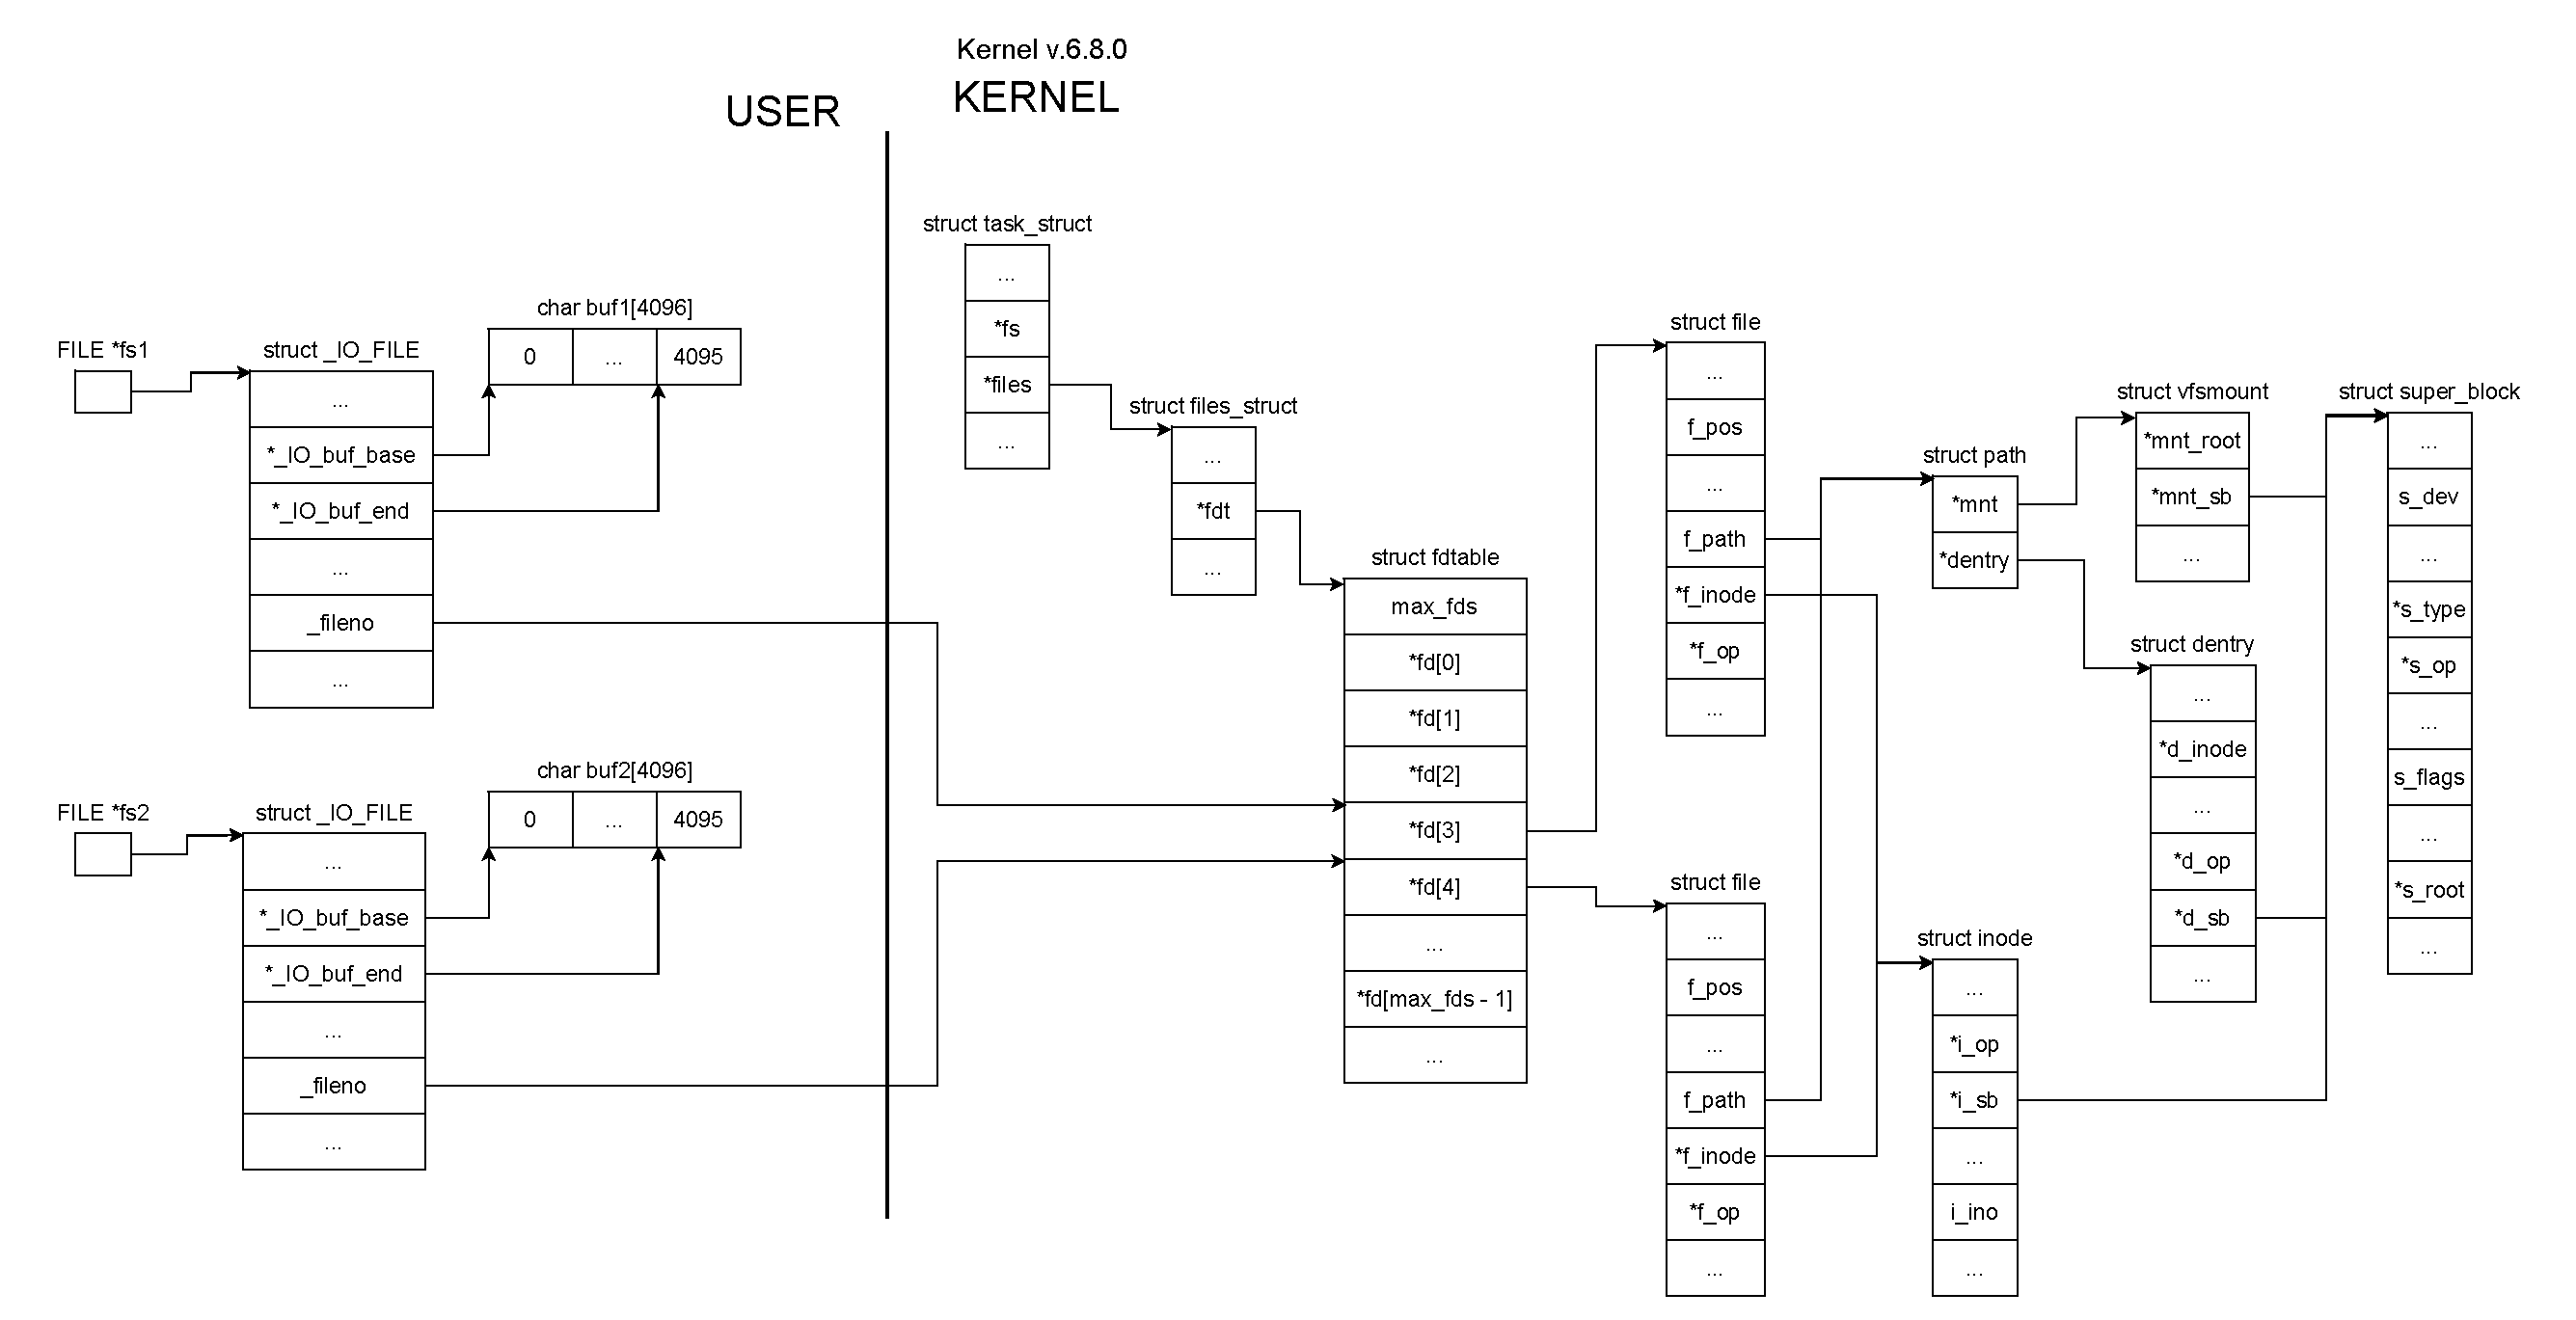
\includegraphics[width=1\textwidth]{3.pdf}
		\caption{Иллюстрация связи структур в третьей программе с fopen, fprintf и fclose}
		\label{pic:scheme_3}
	\end{figure}
\end{document}

